\FloatBarrier

\begin{figure}[h!]
	\centering
	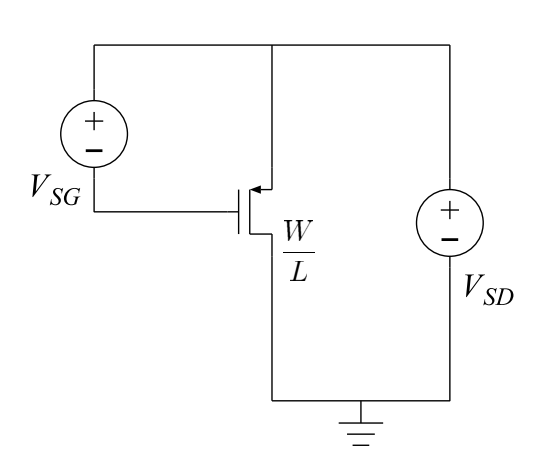
\includegraphics[scale=0.75]{./images/circuit_4.PNG}
	\caption{Circuit 4}
	\label{fig:circuit_4}
\end{figure}

\FloatBarrier

\FloatBarrier

\begin{figure}[h!]
	\centering
	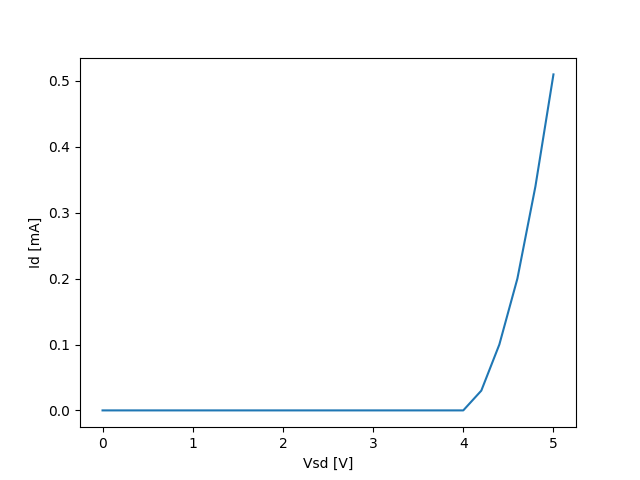
\includegraphics[scale=0.75]{./images/data_4.PNG}
	\caption{$i_{D}$ versus $V_{SD}$ for PMOS with $V_{SG} = 2.5$\si{\volt}}
	\label{fig:data_4}
\end{figure}

\FloatBarrier

One would hope to acquire similar results in figure (\ref{fig:data_4}) for the PMOS as are obtained for the NMOS.
However, the results are drastically different.
Reliable data for the $V_{GS} = 5$\si{\volt} case could not be acquired.
